\chapter{Konzeptionierung des Systems}

Im Rahmen der Konzeptionierung des Systems wurden verschiedene Ideen entwickelt, um das Konzept vom Escape-Room und die Geschicklichkeit des Heißen Draht-Spiels zu kombinieren. Im folgenden werden sechs Konzept vorgestellt, die entwickelt und evaluiert worden sind.

\textbf{Erste Konzept}: Die Spieler des System konnten in verschiedene Rollen schlüpfen. Ein Spieler konnte die Schlaufe nutzen, um das Heiße Draht-Spiel zu spielen und der andere Spieler konnte das gesamte System um die x-Achse sowie die Drähte um die y-Achse rotieren lassen. Zusätzlich hat das System eine Stoppuhr, um die Zeiten zu messen, wie schnell das Spiel durchgespielt werden konnte. Dies sollte für den Wettbewerbsaspekt sorgen. In der Mitte des Systems wurde ein Chip angebracht, um das gesamte System zu steuern. Die Schwierigkeit für den Spiel mit der Schlaufe konnte durch die Größe der Schlaufe angepasst werden. Dieses Konzept wurde,jedoch verworfen das sie das Wesen eines Escape Rooms nicht widerspiegeln konnte. Der Entwurf des Systems sah wie folgt aus: 


\begin{figure}[H]
 \centerline{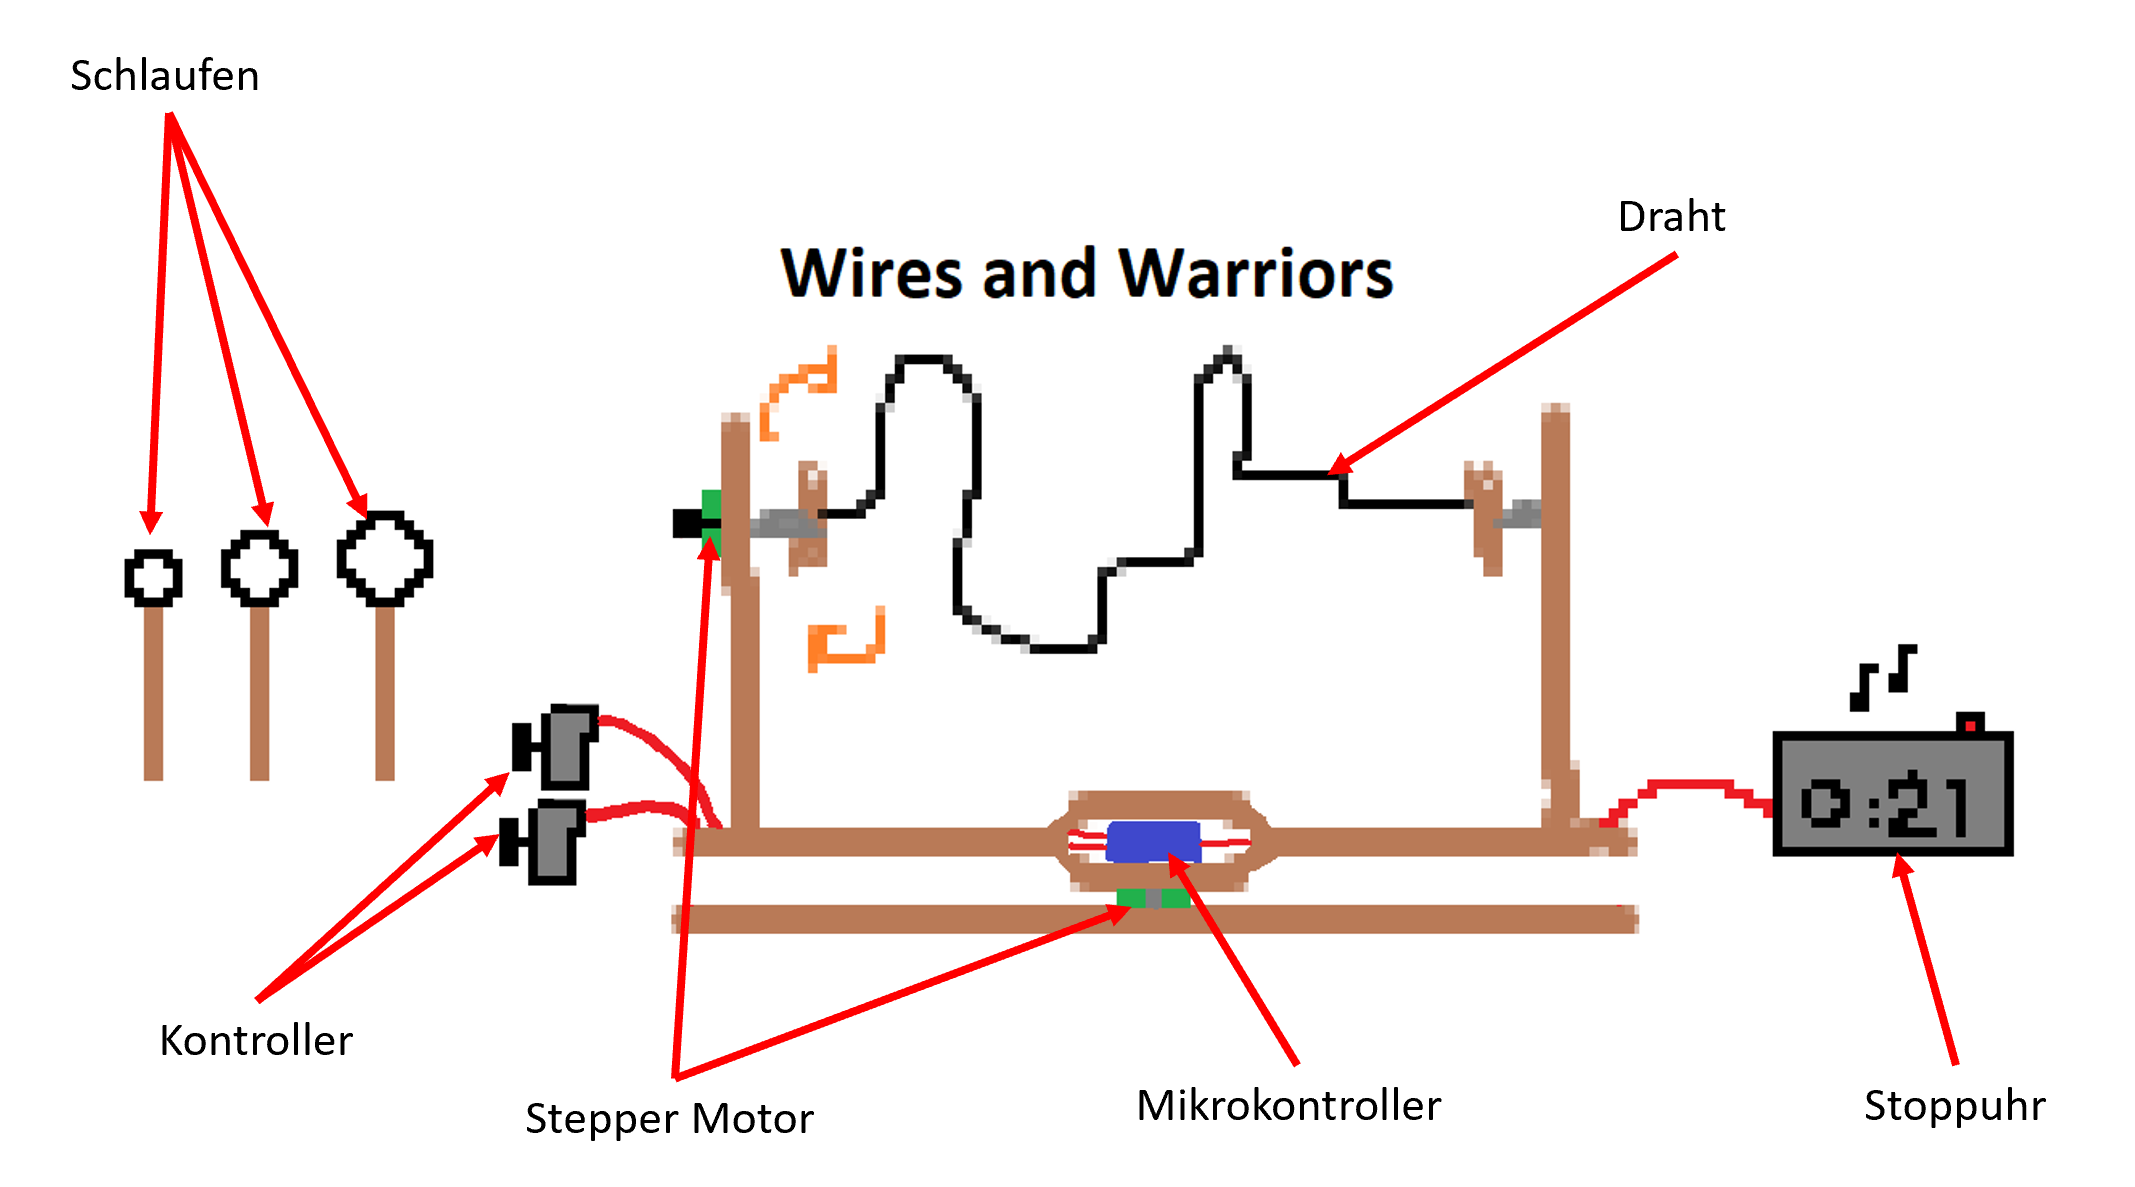
\includegraphics[width=0.75\textwidth,scale=1]{./images/Konzeptpapier_1.png}}
 \caption{Visualisierung des ersten Konzepts}\label{imageLabel}
\end{figure}  

\textbf{Zweite Konzept}: Dieses System sollte drei separate Drähte nutzen: einer rechts, einer links und einer in der Mitte als Brücke. Die äußeren Drähte sollten sich um die Y-Achse und das Mittelstück um die X-Achse drehen können. Das Ziel ist es gewesen, die gegenüberliegende Seite zu erreichen. Die Herausforderung bestand darin, dass die Spieler sich koordinieren mussten, um das Spiel zu beenden. Dieses Konzept war nicht ausgereift, jedoch bietet sie ein vielversprechendes Grundkonzept für die weitere Entwicklung. Der Entwurf des Systems sah wie folgt aus:

\begin{figure}[H]
 \centerline{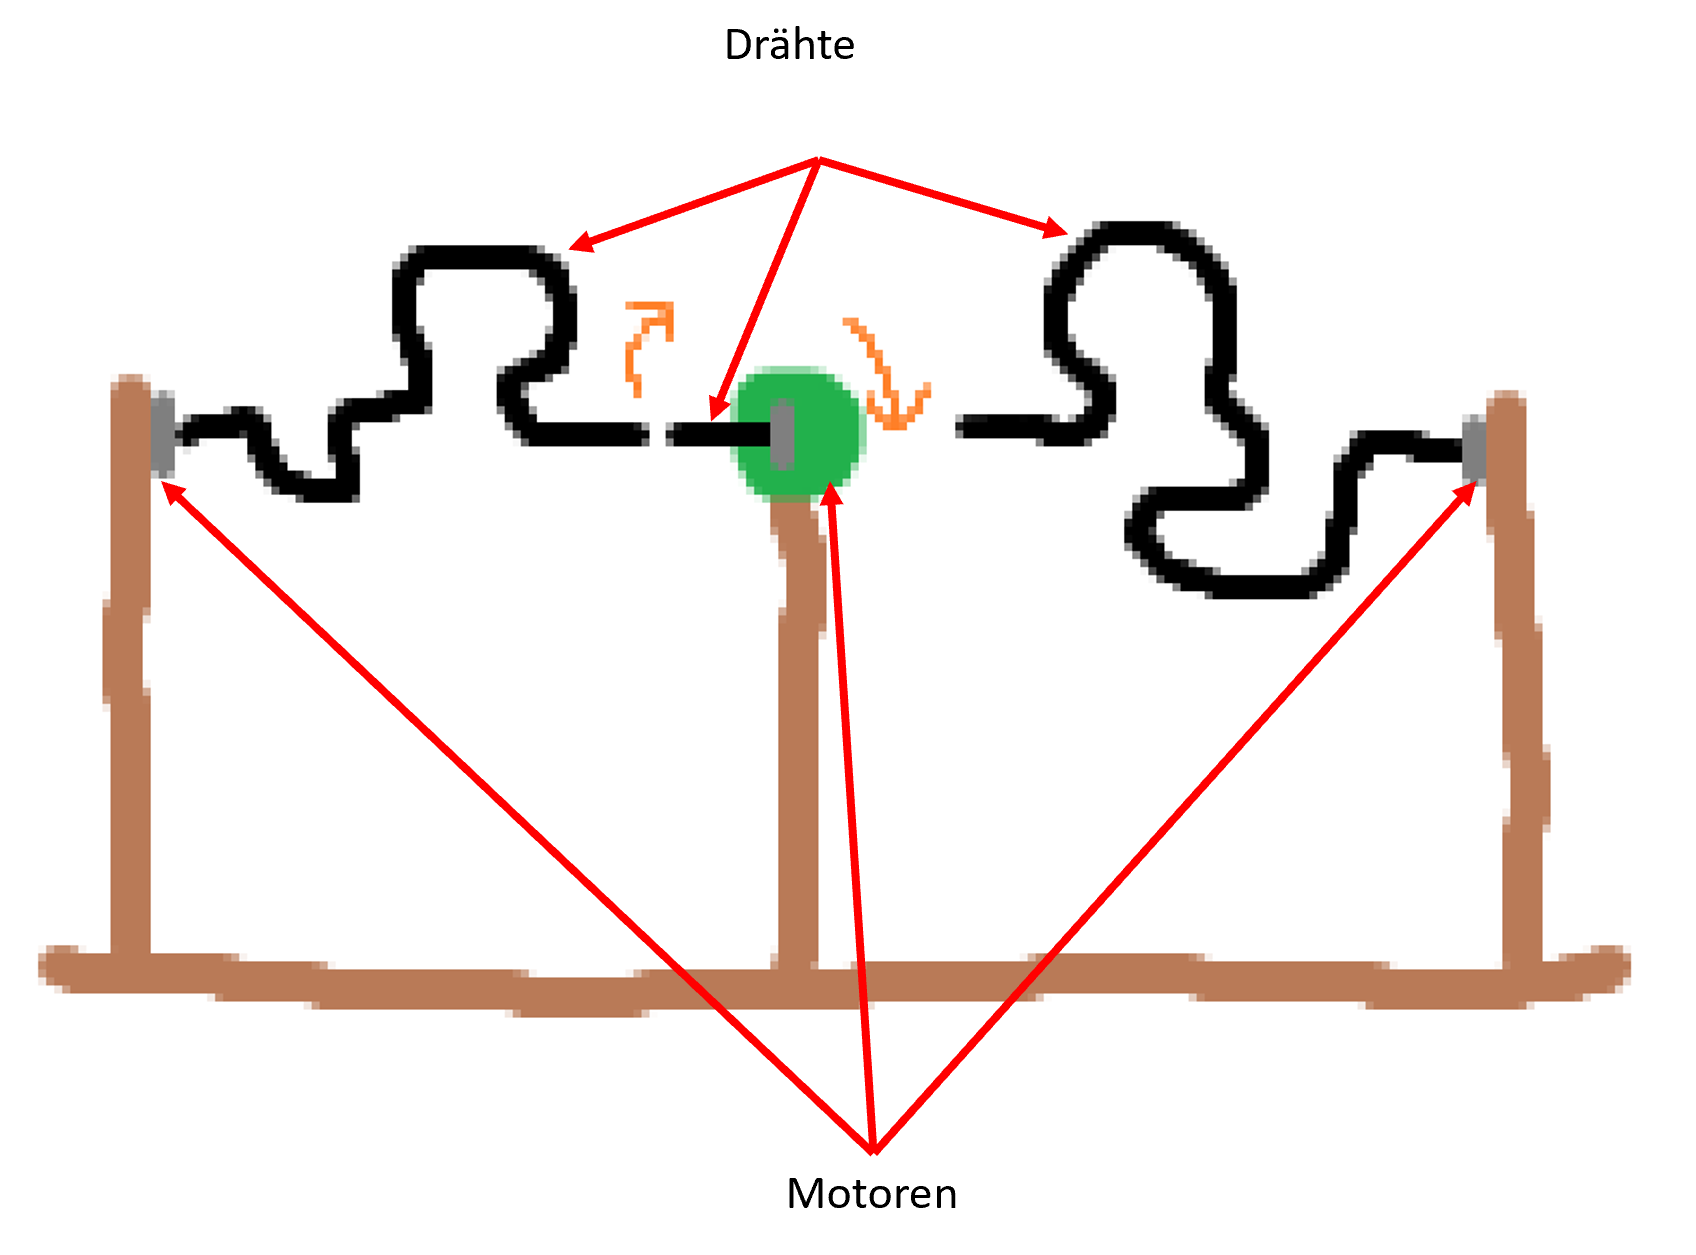
\includegraphics[width=\textwidth,scale=1]{./images/Konzeptpapier_2.png}}
 \caption{Visualisierung des zweiten Konzepts}\label{imageLabel}
\end{figure} 


\textbf{Dritte Konzept}: Das dritte Konzept sollte zwei Drähte besitzen. Diese wurden von den Seiten bis zur Mitte gespannt und am Mittelturm befestigt werden. Beide Spieler mussten, jeweils von den äußeren Seiten in die Mitte gelangen. Es zusätzlich möglich gewesen das ein dritter Spieler das System kontrollieren konnte über Kontroller. Diese Kontroller haben es ihm ermöglicht, die zwei Drähte rotieren zu lassen. Dieses Konzept entsprach nicht dem Charakter eines Escape-Rooms und wurde verworfen. Der Entwurf des Systems sah wie folgt aus: 

\begin{figure}[H]
 \centerline{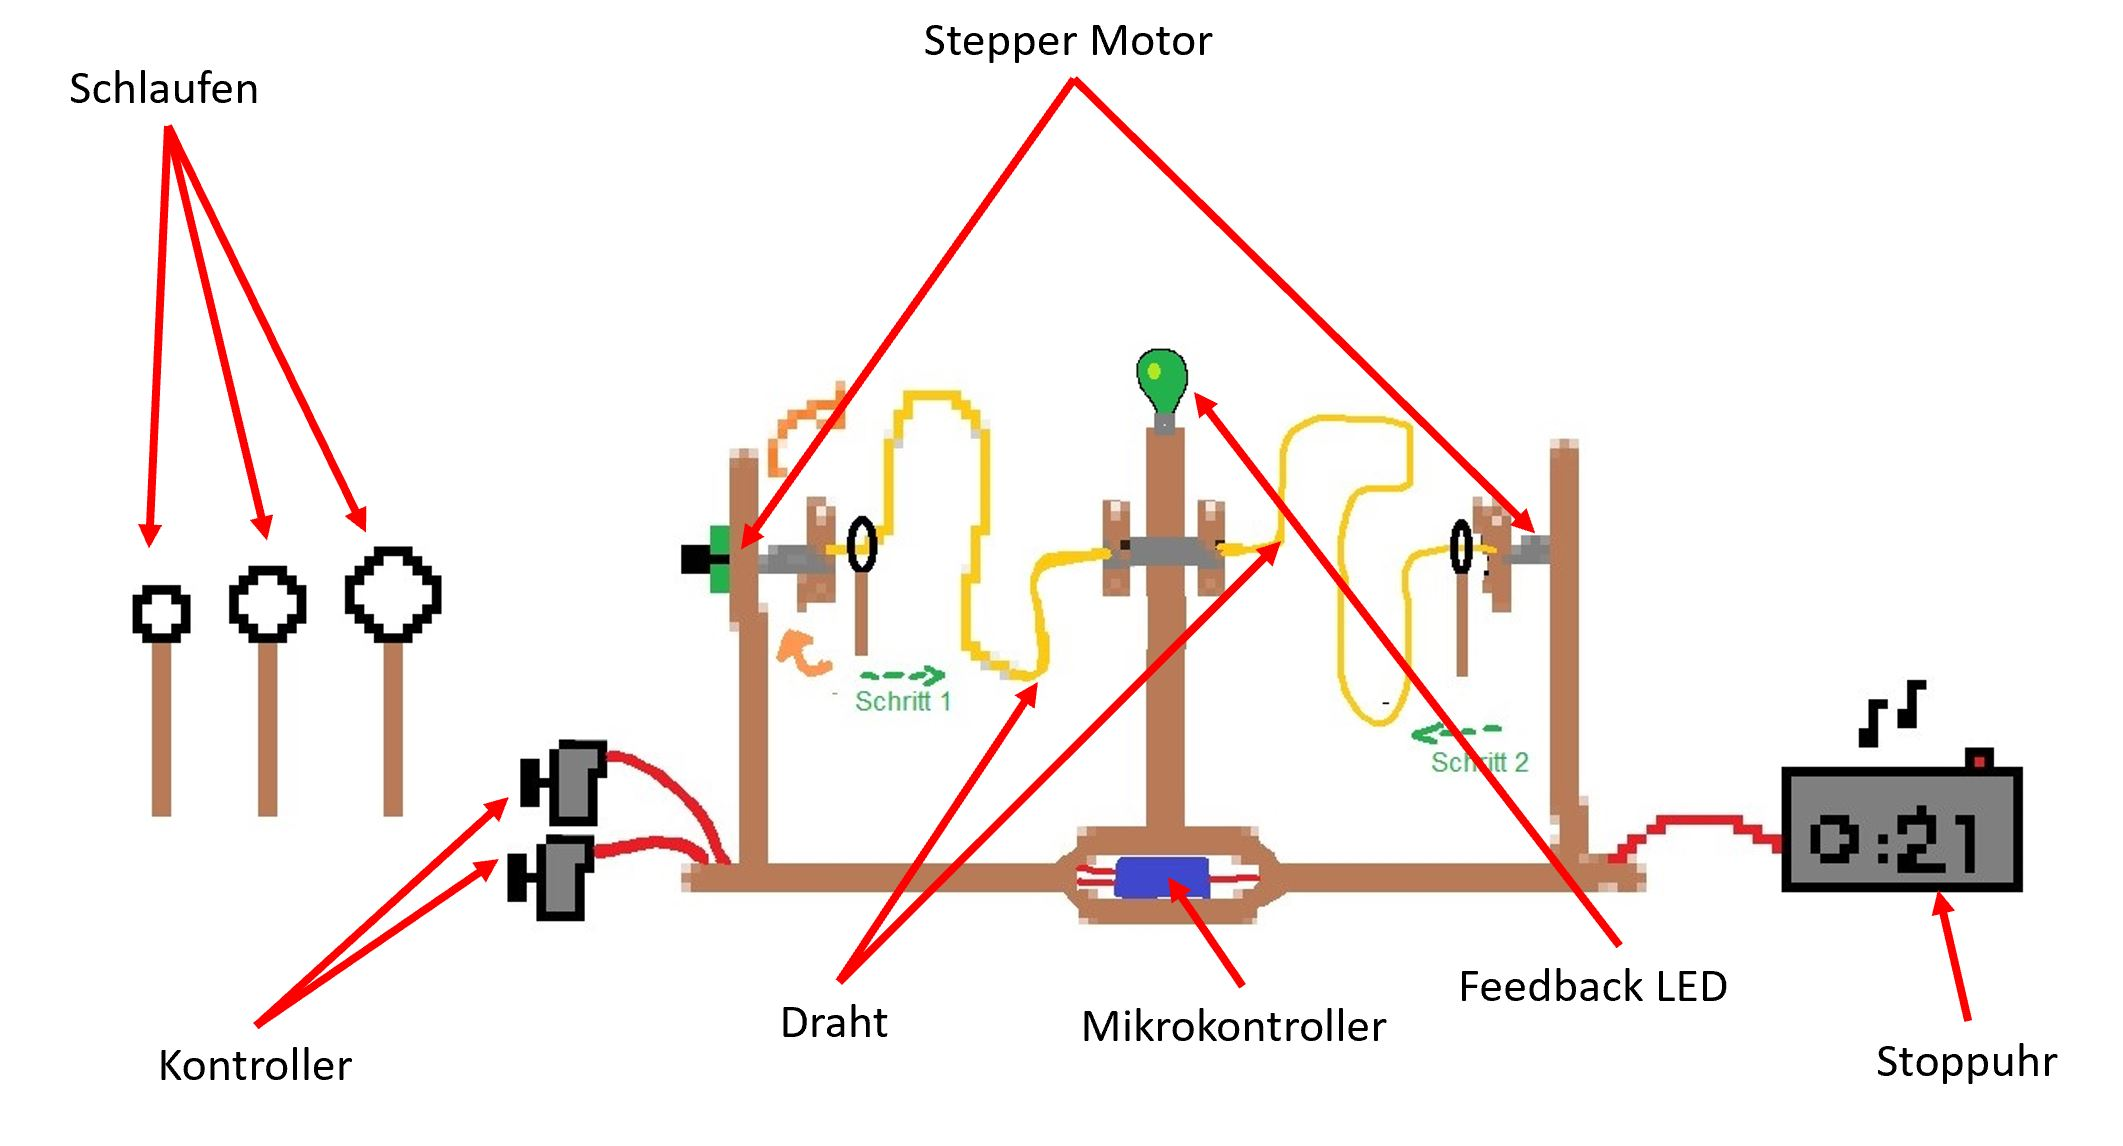
\includegraphics[width=\textwidth,scale=1]{./images/Konzeptpapier_3.jpg}}
 \caption{Visualisierung des dritten Konzepts}\label{imageLabel}
\end{figure} 


\textbf{Vierte Konzept}: Dieses Mal wurden die Türme auf einer Seite und die Brücke gegenüber platziert. Die Drahttürme rotieren um die Y-Achse und die Brücke um die X-Achse. Diese Idee wurde aufgrund mangelnder Nutzerfreundlichkeit schnell verworfen, jedoch wurde das Konzept des äußeren Gerüsts für das finale Design als Basis genutzt. Der Entwurf des Systems sah wie folgt aus:

\begin{figure}[H]
 \centerline{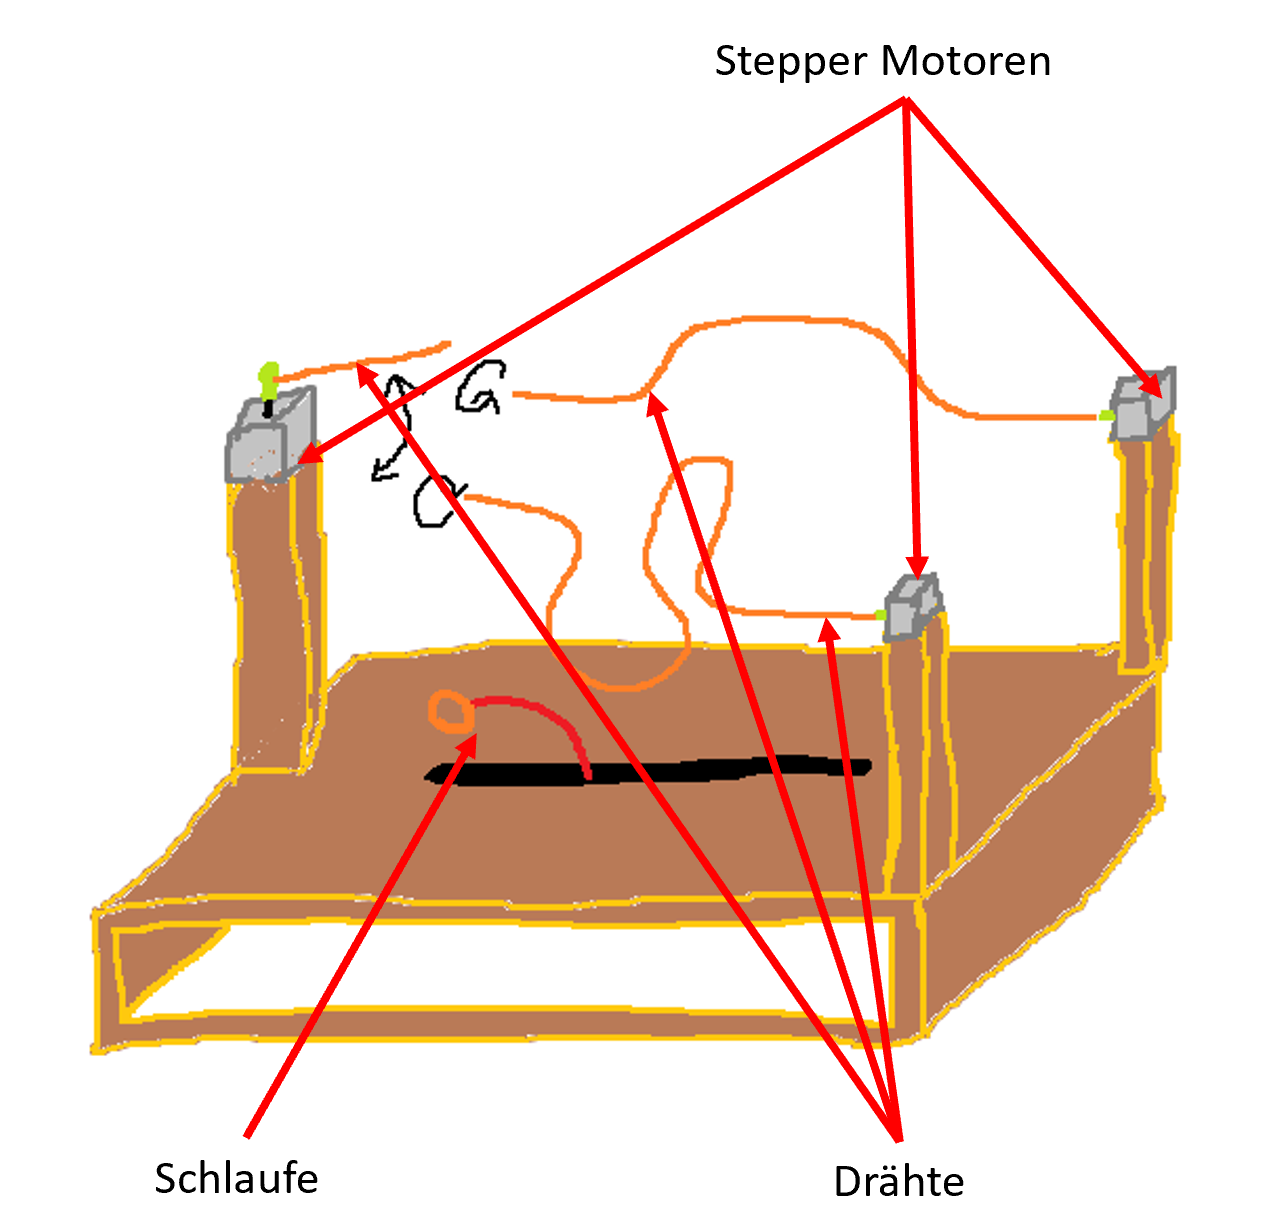
\includegraphics[width=.6\textwidth,scale=1]{./images/Konzeptpapier_6.png}}
 \caption{Visualisierung des vierten Konzepts}\label{imageLabel}
\end{figure} 

\textbf{Fünfte Konzept}: Das letzte Konzept ist eine Kombination aus dem dritten und zweiten Ansatz gewesen. Es gibt zwei Spieler, die gegen das System antreten, mit drei Drähten: links, rechts und ein Mittelstück. Die äußeren Drähte drehen sich um die Y-Achse, das Mittelstück um die X-Achse. Das System sollte Startknöpfe, Fehler-LEDs und Herzen zur Spieler-Rückmeldung besitzen. Die Spieler starten an den äußeren Türmen und müssen auf die andere Seite gelangen. Dieses Konzept war erfolgversprechend und wurde als Grundkonzept genommen und ausgearbeitet. Der Entwurf des Systems sah wie folgt aus:

\begin{figure}[H]
 \centerline{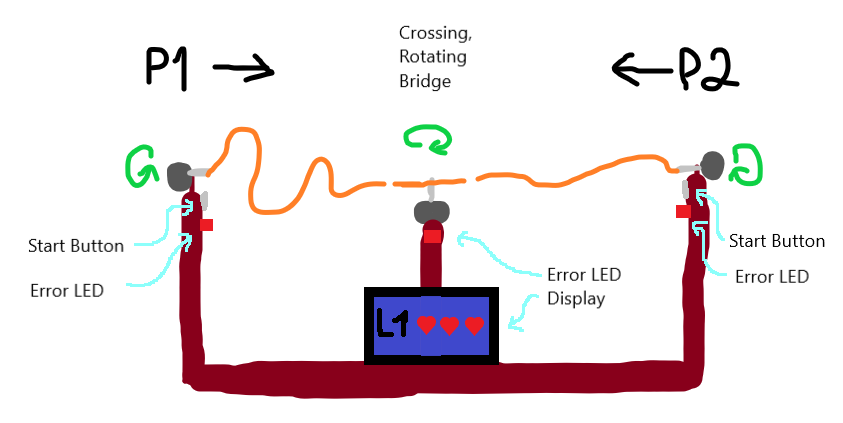
\includegraphics[width=\textwidth,scale=1]{./images/Konzeptpapier_5.png}}
 \caption{Visualisierung des fünfte Konzepts}\label{imageLabel}
\end{figure} 

\section{Modellierung des 3D-Design}

Bei der Modellierung des 3D-Designs für Wire \& Warriors wurde auf ein modulares System geachtet. Die Modularität war ein zentraler Aspekt des Designs, denn dadurch war es möglich die Komponenten für Wartung und Upgrade leicht zugänglich zu machen.

Das gesamte Gerüst des Spieles musste aufgrund der Größenbeschränkung der Holzplatten, jeweils 30x60 Zentimeter groß, durchdacht werden. Die Verwendung von Verzahnung im Modell war ein wichtiger Bestandteil. Diese Bauweise ermöglicht es, dass einzelne Platten fest eineinander greifen konnten, wodurch eine stabile Struktur ohne zusätzliche Verbindungselemente wie Schrauben oder Nägel zu schaffen. Diese Verzahnung sahen wie folgt aus:


\begin{figure}[H]
 \centerline{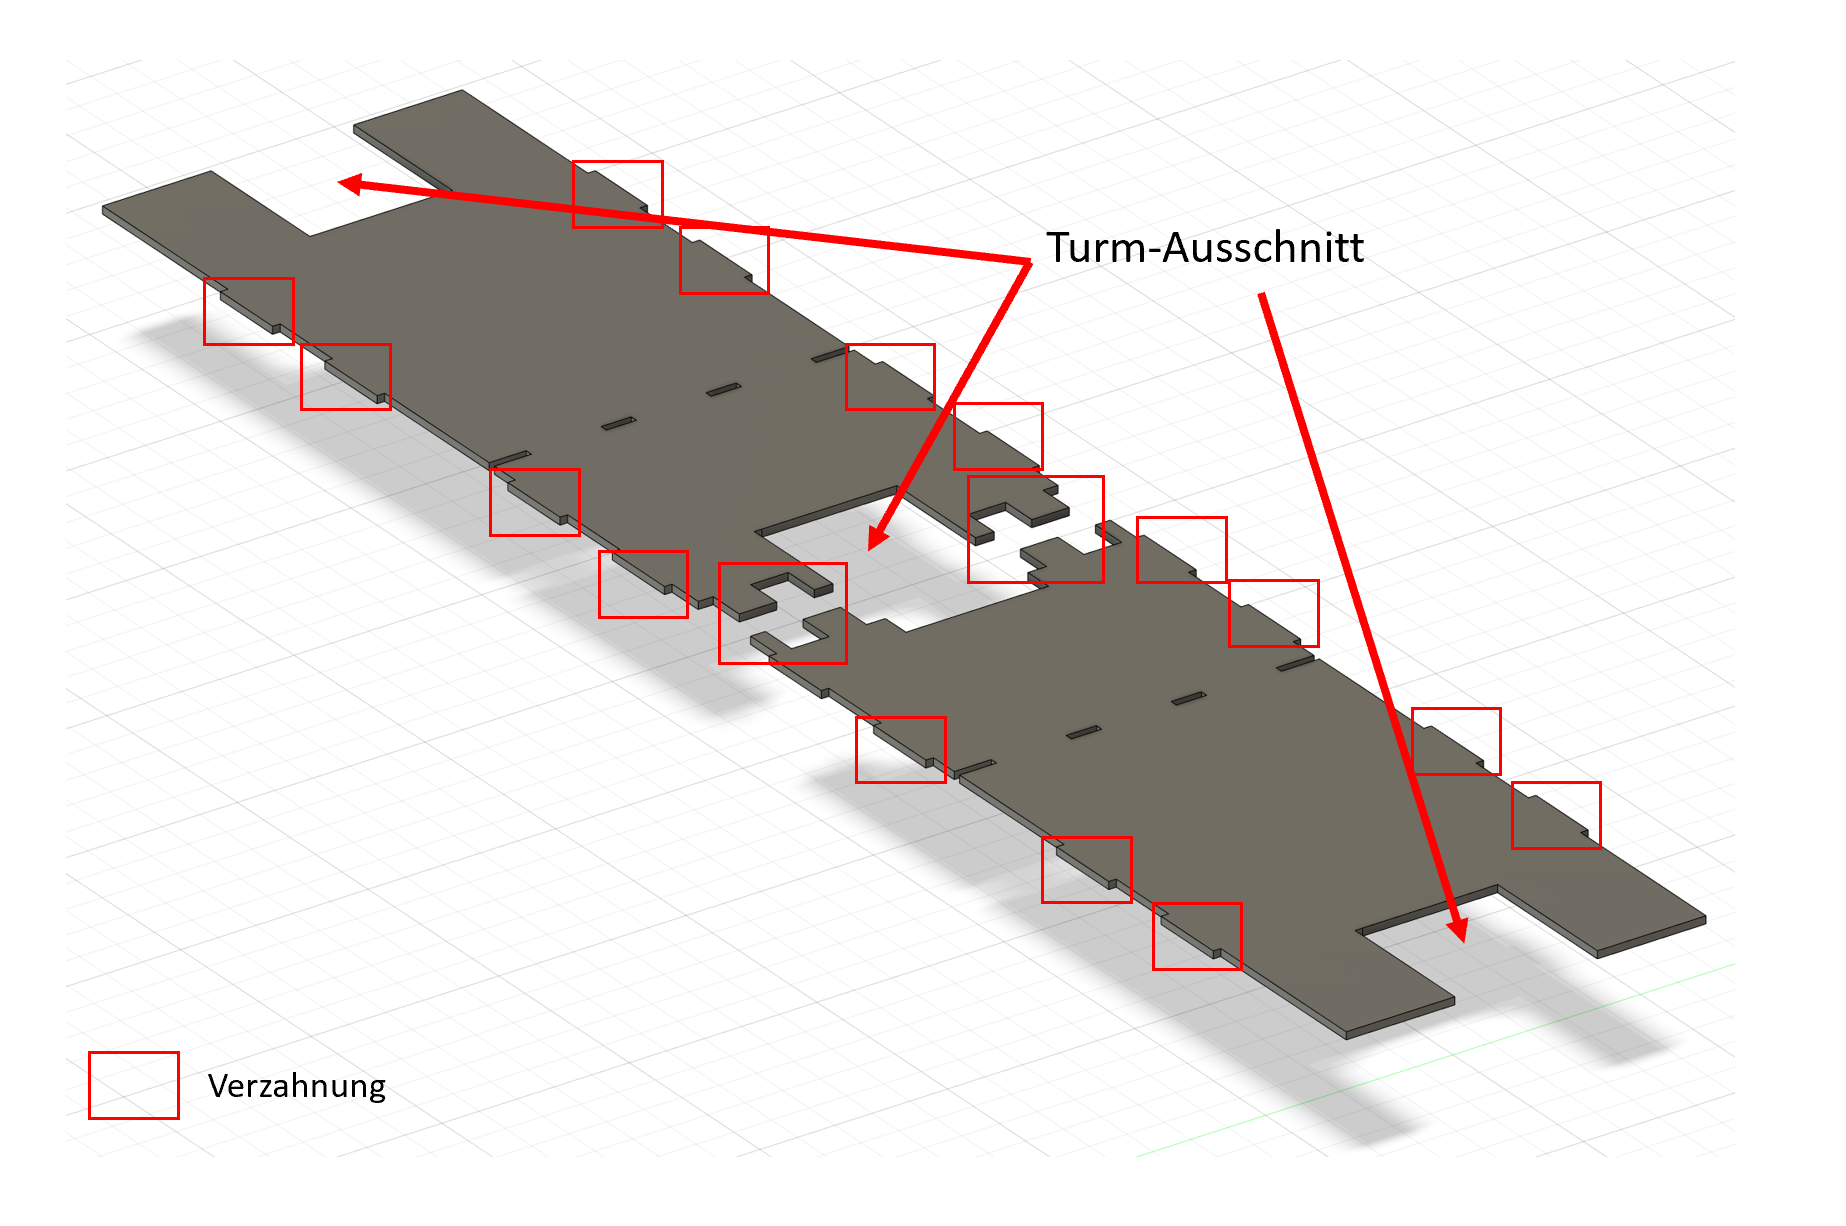
\includegraphics[width=\textwidth,scale=1]{./images/verzahnung.png}}
 \caption{Verzahnung am Deckel}\label{imageLabel}
\end{figure} 

Zusätzlich wurde des gesamt Gerüst durch die Mittelstücke, die auch als Kabelführung gedient haben, verstärkt. Die Mittelstücke wurden im Deckel, in den Wänden und am Boden angebracht. Diese Mittelstücke sehen wie folgt aus:

\begin{figure}[H]
 \centerline{\includegraphics[width=0.75\textwidth,scale=1]{./images/mittelstück.png}}
 \caption{Stabilisierung des Gerüstes durch Mittelstücke}\label{imageLabel}
\end{figure} 

Die Türme des Spieles wurden in das Gerüst eingesetzt und wurden durch die Deckel befestigt. Jeder Turm hatte einen Ausschnitt für den Stepper-Motor und eine Ablage. Die Türme sahen wie folgt aus:

\begin{figure}[H]
 \centerline{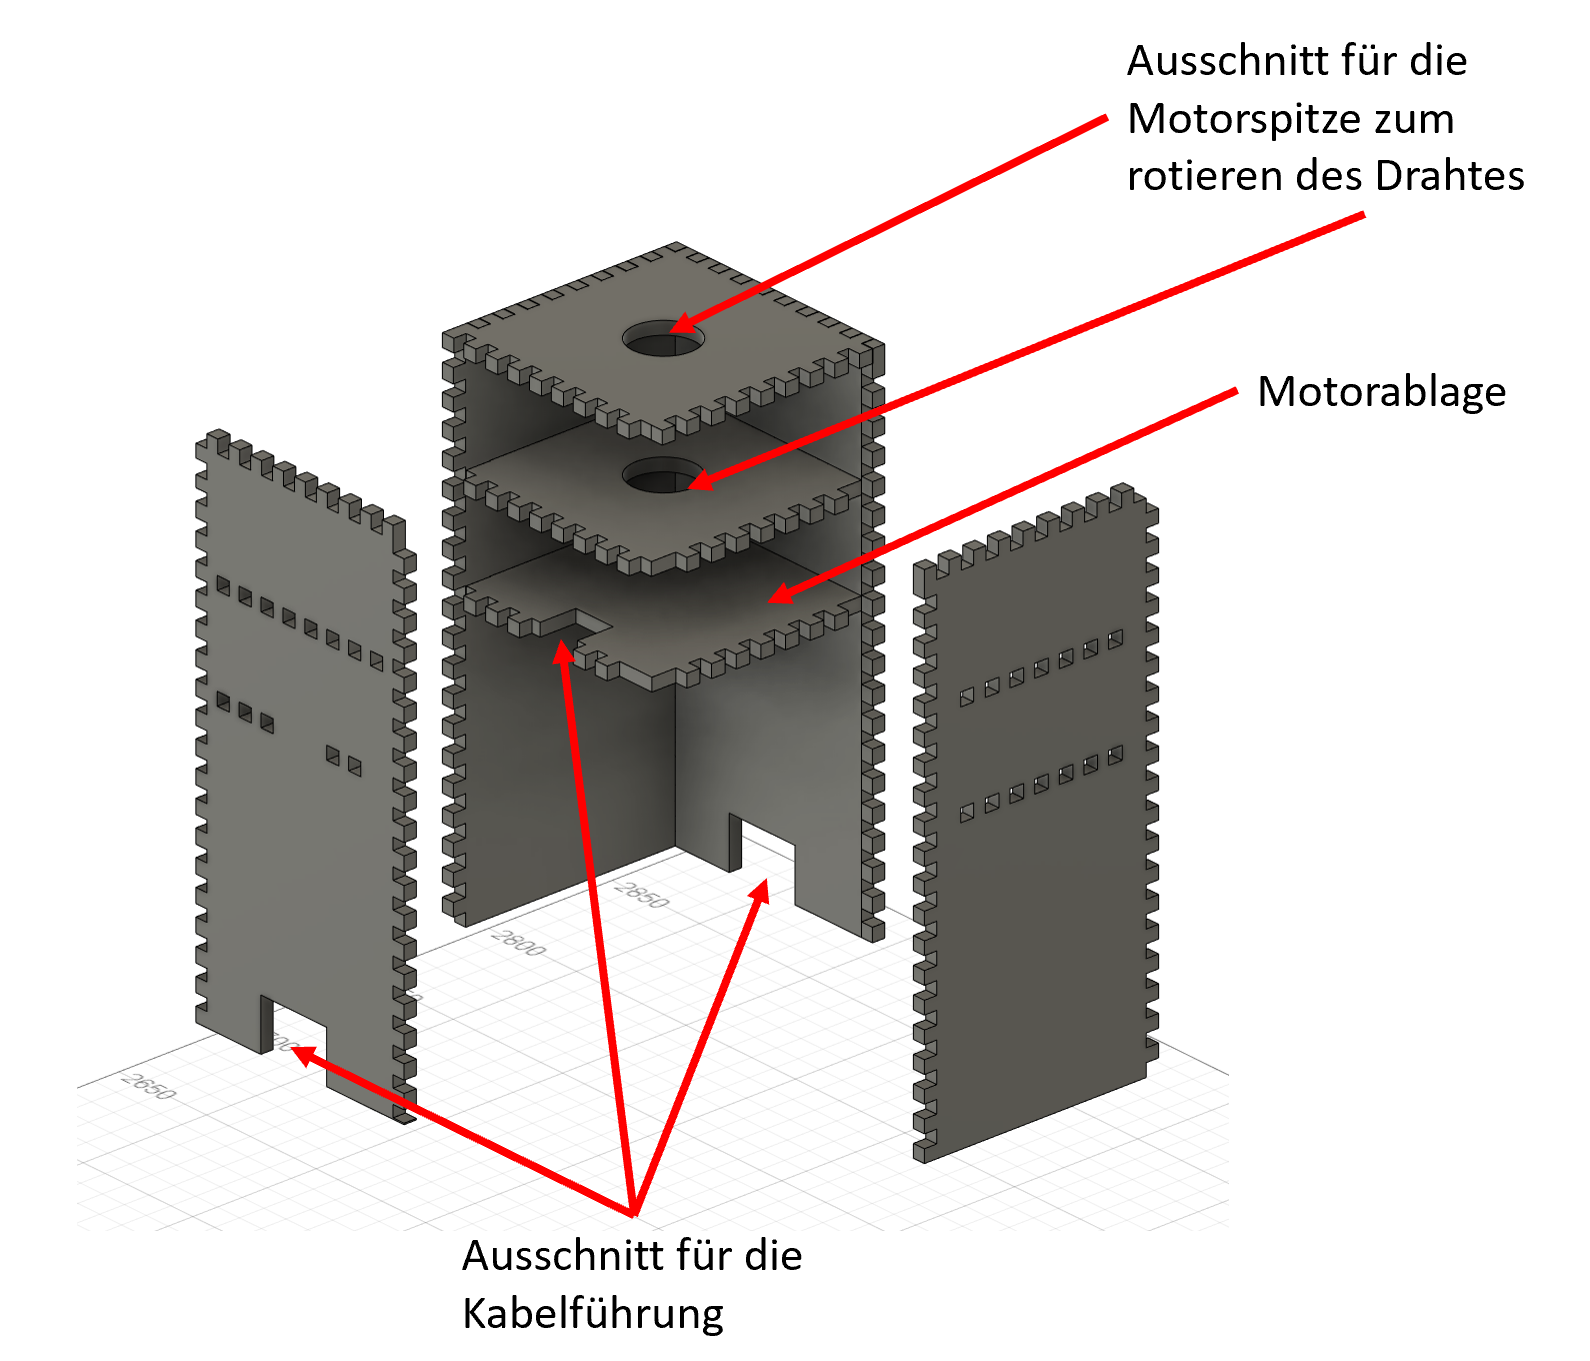
\includegraphics[width=0.75\textwidth,scale=1]{./images/turm_mitte.png}}
 \caption{Einblick in den mittleren Turm}\label{imageLabel}
\end{figure} 


Das gesamte Design diente als Vorlage für die Laserauschnitte, die später aus den Holzplatten gefertigt wurden. Diese Vorbereitung ist entscheidend gewesen, damit alle Teile Präzise zusammenpassen. 

Die Modularität und die leichte Zugänglichkeit der Komponenten sorgt für eine einfach Wartung bzw. Upgrades. Das hat den Vorteil, dass eine schnelle Anpassung z.B. an neue Spielvariaten möglich wäre. Das Endresultat ist ein durchdachtes und funktionales 3D-Design und sieht wie folgt aus: 

\begin{figure}[H]
 \centerline{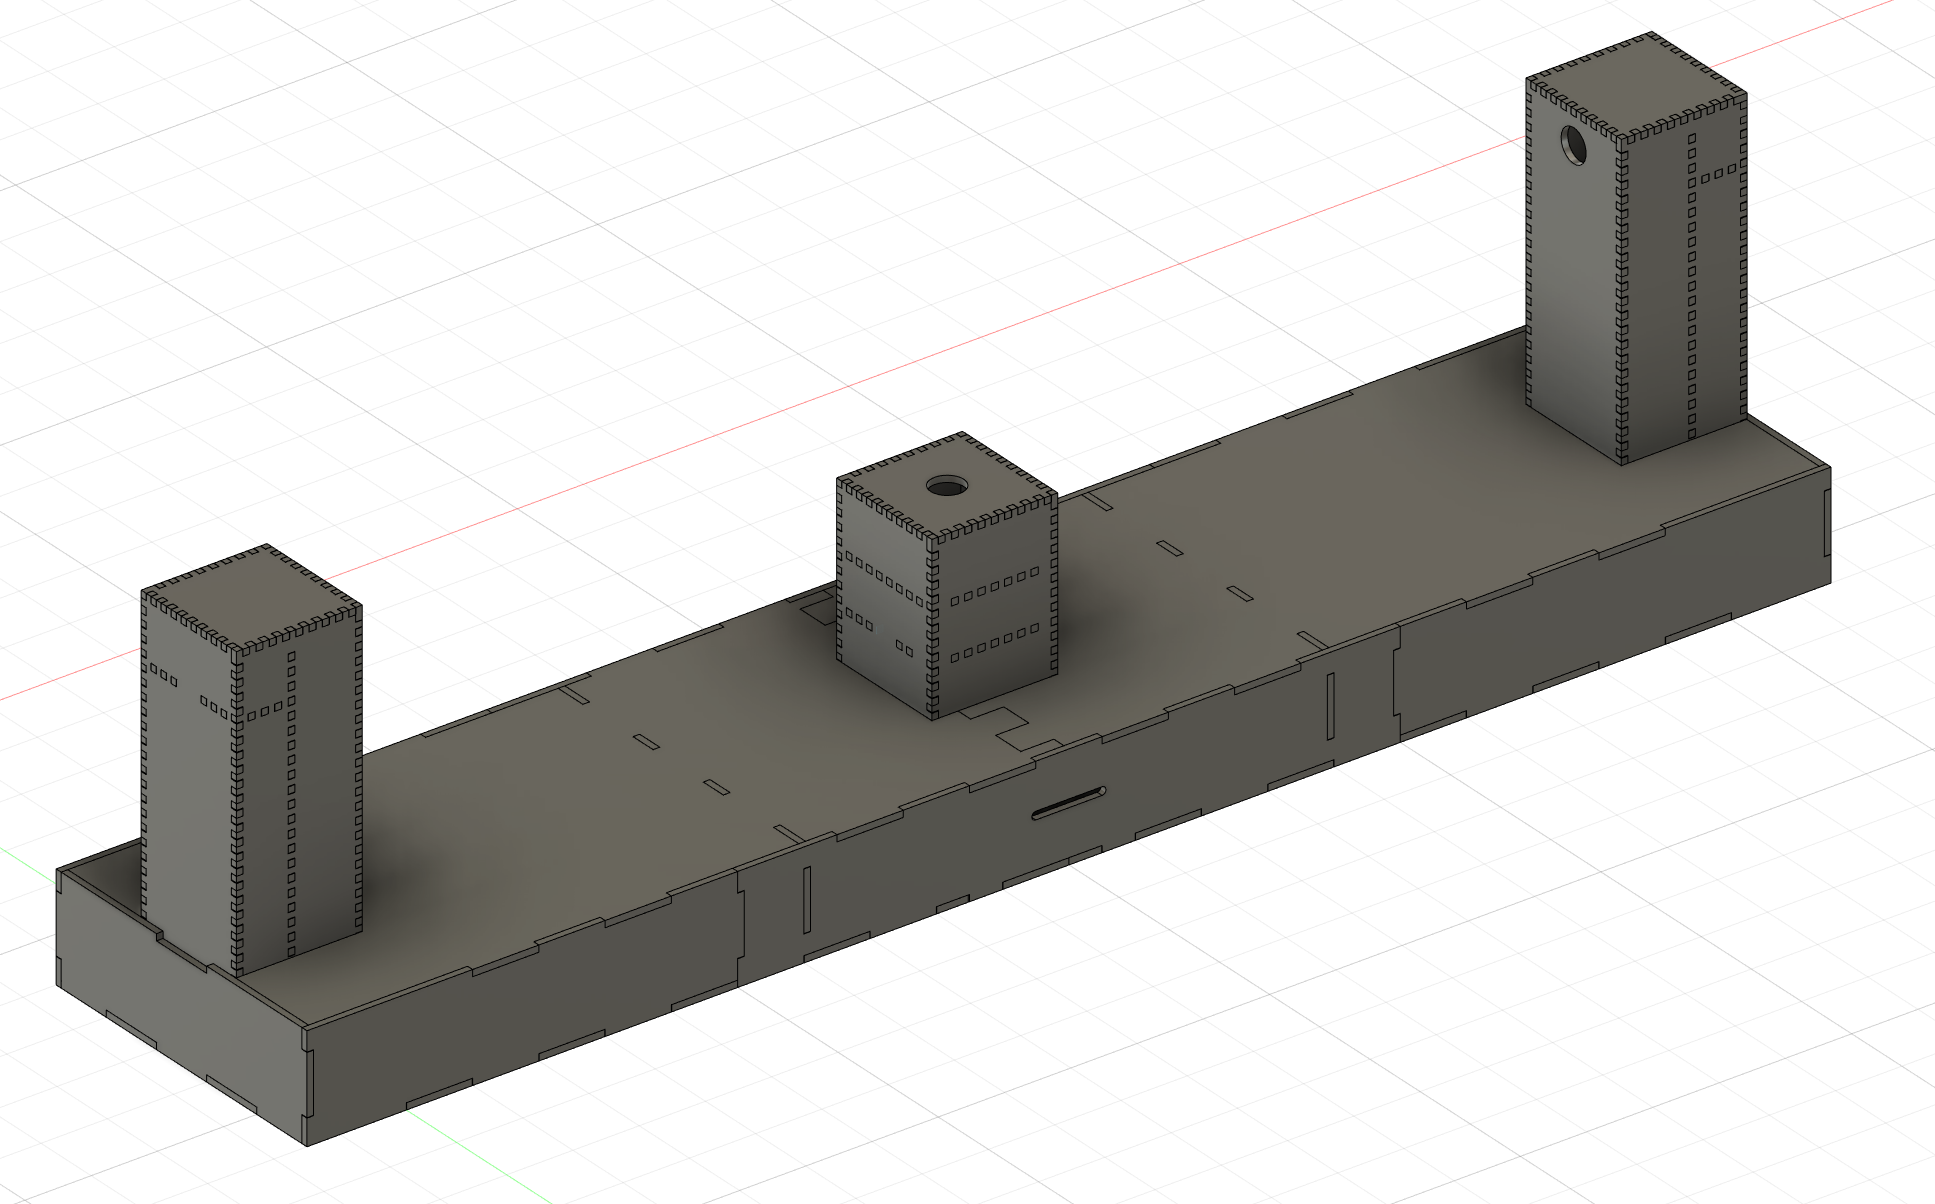
\includegraphics[width=\textwidth,scale=1]{./images/gesamt_design.png}}
 \caption{Das gesamte Design für Wire \& Warriors}\label{imageLabel}
\end{figure} 

